\documentclass{article}
\usepackage{amsmath,amssymb}
\usepackage{graphicx}
\usepackage[top=1in, bottom=1.25in, left=1.25in, right=1.25in]{geometry}

\begin{document}

% ------------------------------------------------------------------------------------------
\section*{Description of the planar torus grid}
% ------------------------------------------------------------------------------------------

\textit{Author 05/2016: F.\ Prill, DWD}

\begin{figure}[ht]
  \centering
  
\includegraphics[width=0.33\textwidth]{torus.pdf}
  \caption{Topological representation of the torus geometry.}
  \label{fig1}
\end{figure}

The torus grid consists of equal-sided triangles, with edge length
\texttt{edge\_length}, which is a namelist parameter of the grid
generator, and height $\frac{\sqrt{3}}{2} \, \texttt{edge\_length}$,
cf. Fig.~\ref{fig2}.


The lon-lat parameterization of the torus is 
\begin{align*}
  (lon,lat) = [0, 2 \, \pi]  \times [- \texttt{max\_lat}, \texttt{max\_lat}]
\end{align*}
where $\texttt{max\_lat} := \frac{\pi}{18} \equiv 10~ \text{degrees}$
(hard-coded in the torus grid generator).  Variables related to the
lon-lat parameterization are stored as the data type
\texttt{t\_geographical\_coordinates} in the ICON code.

The Cartesian coordinates of the torus grid are: $v = (x,y,0)$
where
\begin{align*}
   (x,y) = [0,\texttt{domain\_length}] \times [0,\texttt{domain\_height}]
\end{align*}
The lengths \texttt{domain\_length}, \texttt{domain\_height} are
stored as global attributes in the grid file.  Related to the namelist
parameters \texttt{x\_no\_of\_columns}, \texttt{y\_no\_of\_rows}
of the grid generator we have
\begin{itemize}
 \item \texttt{domain\_length} := \texttt{edge\_length * x\_no\_of\_columns}
 \item \texttt{domain\_height} := $\frac{\sqrt{3}}{2}$ \texttt{ * edge\_length y\_no\_of\_rows}
\end{itemize}

Variables related to the Cartesian mesh are stored as the data type
\texttt{t\_cartesian\_coordinates} in the ICON code.

\begin{paragraph}{Note}
  The torus geometry and the corresponding global meta-data (NetCDF attributes)
  are \emph{not} generated by the ''standard grid generator''
  in \texttt{src/grid\_generator}, but require L.\ Linardakis' grid generator
  tool (e.\,g.\ available in \texttt{branches/icon-test-torus}).
\end{paragraph}

\begin{figure}[ht]
  \centering
  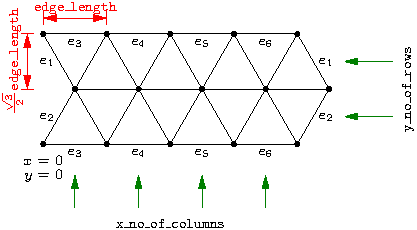
\includegraphics[width=0.6\textwidth]{torus_plane.pdf}
  \caption{Triangulation of the torus mesh.}
  \label{fig2}
\end{figure}



\end{document}
